\documentclass[11pt]{article}

\usepackage[margin=1in]{geometry}
\usepackage{amsmath,amssymb}
\usepackage{graphicx}
\usepackage{booktabs}
\usepackage{xcolor}
\usepackage{hyperref}
\usepackage{microtype}

\graphicspath{{../paper_drafts/figures/}}

\newcommand{\dabe}{\textsc{DABE}}
\newcommand{\Exp}[1]{\textsc{EXP-#1}}
\newcommand{\bitsper}{bits/token}
\newcommand{\Vocab}{\mathcal{V}}
\newcommand{\indicator}{\mathbb{1}}
\newcommand{\softmax}{\operatorname{softmax}}
\newcommand{\TopK}{\operatorname{TopK}}
\newcommand{\CE}{\operatorname{CE}}

\title{Density-Adaptive Bitmask Encoding: Fixed Chunks with Sparse Lexical Repair}
\author{
Mainasara Al-amin Tsowa\\
\texttt{mainasara@qrk.ng}
\and
Babangida Usman Tsowa\\
\texttt{babangida@qrk.ng}
}
\date{}

\begin{document}
\maketitle

\begin{abstract}
Modern subword tokenizers are efficient and robust, but they allocate lexical capacity through a fixed segmentation policy rather than through the local information demand of a span. We study Density-Adaptive Bitmask Encoding (\dabe), a learned tokenizer-autoencoder that compresses fixed 64-token chunks into binary codes and spends additional sparse lexical repair capacity only where reconstruction is difficult.

Across TinyStories tokenizer-autoencoder experiments, we find that the most effective design is not adaptive token-window geometry. Instead, a stable fixed chunk paired with a coarse gist stream and a residual-routed sparse lookup stream gives the best rate-distortion tradeoff. The best quality setting reaches 0.91547 token accuracy and 5.41007 mean chunk deviation at 20.37236 observed \bitsper. A replicated cost-aware setting identifies \texttt{lookup\_slot\_cost\_weight=0.025} as a local compression knee, reaching 0.89274 token accuracy and 6.86454 mean chunk deviation at 20.06207 observed \bitsper.

Controlled ablations show that sliding or variable token windows either reduce bitrate at substantial reconstruction cost or collapse to all-fine routing. A matched fixed-rate no-lookup baseline at 20.0 \bitsper\ reaches only 0.72045 token accuracy and 17.89119 mean chunk deviation, compared with the cost-aware \dabe\ point's 0.89274 token accuracy and 6.86454 mean chunk deviation at 20.06207 observed \bitsper. These results identify stable chunks plus adaptive repair as the stronger learned-tokenizer mechanism at matched bitrate.
\end{abstract}

\section{Introduction}
Subword tokenizers define the discrete interface between text and modern language models. Before a model sees language, text is committed to a sequence of symbols chosen by a tokenizer, usually a subword segmentation scheme such as byte-pair encoding or a related unigram model \cite{sennrich2016bpe,kudo2018sentencepiece}. These methods are efficient, robust, and easy to deploy, but their rate allocation is primarily corpus-level: frequent fragments receive compact symbols, rare lexical details are decomposed into longer sequences, and local span difficulty is not represented as an explicit allocation decision.

Natural text has nonuniform information density. A span may contain predictable function words, repeated narrative scaffolding, rare names, punctuation-sensitive dialogue, or local details that are easy to paraphrase but hard to reconstruct exactly. This creates a tokenizer-level rate-distortion question: which parts of a span require lexical precision, and which parts can be represented by a coarse semantic gist?

We study this question through \dabe, a learned tokenizer-autoencoder that compresses fixed 64-token chunks into binary codes and reconstructs the original token sequence. The goal is not merely to replace one vocabulary with another. Instead, \dabe\ treats tokenization as a rate-distortion problem: given a finite bit budget, how should a learned tokenizer allocate capacity across a span so that reconstruction error falls where it matters most?

The central design choice in this work is to decouple coarse meaning from lexical repair. A \dabe\ chunk first receives a compact gist representation intended to capture broad local structure. A second, sparse repair pathway then allocates additional lexical lookup capacity to positions predicted to be difficult. This produces a sliding repair budget over a stable chunk, rather than a sliding token window. The distinction matters: changing the primary token-window geometry can reduce nominal bitrate, but it can also disrupt local code specificity and make reconstruction brittle. In contrast, keeping the chunk stable while adapting the repair budget lets the model preserve a consistent coarse representation and spend precision only where residual error suggests it is useful.

Our experiments on TinyStories establish this framing empirically. The strongest setting, a fixed 64-token chunk with gist encoding and residual-routed sparse lexical lookup, reaches 0.91547 token accuracy and 5.41007 mean chunk deviation at 20.37236 observed \bitsper. A cost-aware operating point replicated across adjacent cost settings reaches 0.89274 token accuracy and 6.86454 mean chunk deviation at 20.06207 observed \bitsper. A matched fixed-rate no-lookup baseline at 20.0 \bitsper\ is stable and non-collapsed, but reaches only 0.72045 token accuracy and 17.89119 mean chunk deviation. The result is a matched-rate separation: the gain is not explained by total bit budget alone, but by the model's ability to place lexical precision where reconstruction requires it.

This paper makes four contributions:
\begin{itemize}
  \item We formulate \dabe\ tokenization as a learned rate-distortion problem over fixed token chunks, with binary codes and explicit reconstruction metrics.
  \item We introduce a gist-plus-residual-repair architecture that separates coarse span representation from sparse lexical precision.
  \item We show that adaptive sparse repair substantially outperforms a matched fixed-rate no-lookup learned tokenizer at approximately 20 \bitsper.
  \item We provide controlled ablations showing that adaptive token-window geometry is not, by itself, the right mechanism for this setting.
\end{itemize}

The paper therefore makes a specific rate-distortion claim: within a controlled tokenizer-autoencoder setting, adaptive sparse lexical repair over stable chunks gives a stronger reconstruction frontier than either fixed-rate learned compression or adaptive token-window geometry. This is the mechanism result that future full language-model integration should build on.

\section{Related Work}
\paragraph{Subword tokenization.}
Most contemporary language models use fixed tokenization policies such as byte-pair encoding, WordPiece, unigram language-model tokenization, or byte-level variants \cite{sennrich2016bpe,kudo2018sentencepiece,schuster2012japanese}. These methods are robust and efficient, but they allocate sequence length through corpus-level frequency statistics rather than through the local information density of a span. \dabe\ keeps the deployment motivation of compact discrete representations, but studies whether a learned tokenizer can allocate reconstruction capacity adaptively inside a fixed chunk.

\paragraph{Learned discrete tokenizers.}
Discrete autoencoders, vector-quantized models, residual quantizers, and semantic hashing methods learn compact latent codes that can reconstruct or represent text \cite{vandenoord2017vqvae,kaiser2018discrete}. These approaches motivate treating tokenization as a learned compression problem rather than a fixed segmentation problem. The fixed-rate no-lookup \dabe\ baselines in \Exp{071}, \Exp{079}, and \Exp{093} play this role in our experiments: they ask how much reconstruction quality a learned chunk code obtains when it spends all capacity uniformly.

\paragraph{Adaptive computation and routing.}
Adaptive computation mechanisms spend more computation on difficult examples, tokens, or positions \cite{graves2016act,bengio2013estimating}. \dabe\ applies the same broad principle to tokenizer reconstruction capacity: the model predicts where sparse lexical repair is worth spending after producing a coarse gist of the chunk. This differs from adaptive windowing because the primary chunk geometry remains stable while the repair budget changes.

\paragraph{Retrieval, copy, and lexical memory.}
Copy and retrieval mechanisms are often used to recover rare or exact lexical details that parametric sequence models blur \cite{gu2016copy,guu2020realm}. \dabe{}'s sparse lexical lookup stream plays a similar role inside the tokenizer itself: it gives the decoder a small budget for high-precision lexical holes while leaving easier positions to the gist representation.

\section{Method}
\subsection{Problem Setup}
Let a tokenized text chunk be
\begin{equation}
  x = (x_1, \ldots, x_T), \qquad x_i \in \Vocab, \qquad T = 64.
\end{equation}
The tokenizer-autoencoder maps this chunk into a binary code and reconstructs a distribution over the original GPT-2 token IDs. We treat the system as a rate-distortion model. A method is useful only when it reduces reconstruction distortion at a comparable observed bitrate.

\subsection{Fixed-Rate Chunk Code}
The learned chunk encoder produces a binary representation
\begin{equation}
  b = q_\phi(x), \qquad b \in \{0,1\}^{B},
\end{equation}
where $B$ is the base code size. The fixed-rate no-lookup comparator reconstructs directly from this code:
\begin{equation}
  h_i = F_\theta(b, i), \qquad
  \ell_i^{\mathrm{base}} = W_o h_i, \qquad
  p_i^{\mathrm{base}} = \softmax(\ell_i^{\mathrm{base}}).
\end{equation}
The fixed-rate bitrate is therefore
\begin{equation}
  R_{\mathrm{fixed}} = \frac{B}{T}.
\end{equation}
For \Exp{093}, $B=1280$ and $T=64$, giving exactly 20.0 \bitsper. This is the matched learned-compression baseline for the cost-aware \dabe\ point.

\subsection{Gist Stream}
The \dabe\ decoder separates coarse reconstruction from sparse repair. First, a gist decoder maps the binary code into position-wise hidden states and logits:
\begin{align}
  g_i &= G_\theta(b, i), \\
  \ell_i^{\mathrm{gist}} &= W_g g_i, \\
  p_i^{\mathrm{gist}} &= \softmax(\ell_i^{\mathrm{gist}}).
\end{align}
This stream is responsible for predictable local structure. It should recover easy tokens without spending lexical lookup slots everywhere.

\subsection{Residual Difficulty Signal}
The residual router estimates where the gist stream is likely to be wrong. In supervised analysis this difficulty can be written as the per-position gist loss
\begin{equation}
  d_i = \CE(x_i, p_i^{\mathrm{gist}}) = -\log p_i^{\mathrm{gist}}(x_i).
\end{equation}
During decoding, the router uses available hidden features rather than ground-truth labels:
\begin{equation}
  r_i = f_\psi(g_i), \qquad r_i \in \mathbb{R}^{K_{\max}},
\end{equation}
where $K_{\max}$ is the maximum number of lexical repair slots that could be exposed for a position or local region. The experiments with residual-router supervision train these scores to correlate with reconstruction difficulty, so high-information holes receive more repair capacity.

\subsection{Sparse Lexical Reconstruction}
Sparse lexical lookup augments the gist logits with a small set of candidate repair vectors. Let
\begin{equation}
  m_{i,k} \in \mathbb{R}^{|\Vocab|}, \qquad k = 1, \ldots, K_{\max}
\end{equation}
be the logit-space contribution of lookup slot $k$ at position $i$. The router converts scores into keep probabilities
\begin{equation}
  a_{i,k} = \sigma(r_{i,k}), \qquad a_{i,k} \in [0,1],
\end{equation}
and the discrete active-slot mask is
\begin{equation}
  z_{i,k} = \indicator[a_{i,k} > \tau].
\end{equation}
The repaired reconstruction logits are
\begin{equation}
  \ell_i^{\mathrm{repair}}
  = \ell_i^{\mathrm{gist}} + \lambda_{\mathrm{lookup}} \sum_{k=1}^{K_{\max}} z_{i,k} m_{i,k},
\end{equation}
and the final token distribution is
\begin{equation}
  p_i^{\mathrm{repair}} = \softmax(\ell_i^{\mathrm{repair}}).
\end{equation}
This equation is the core sparse-reconstruction claim: the binary chunk code supplies a smooth whole-span gist, while the lookup path fills a small number of lexical holes selected by the residual router.

\subsection{Cost-Aware Objective}
The reconstruction objective is token cross-entropy over the repaired distribution:
\begin{equation}
  \mathcal{L}_{\mathrm{rec}}
  = \frac{1}{T} \sum_{i=1}^{T} \CE(x_i, p_i^{\mathrm{repair}}).
\end{equation}
Cost-aware runs add a penalty for using lookup capacity:
\begin{equation}
  \mathcal{L}
  = \mathcal{L}_{\mathrm{rec}}
  + \alpha_{\mathrm{slot}} \frac{1}{T K_{\max}} \sum_{i=1}^{T} \sum_{k=1}^{K_{\max}} a_{i,k}
  + \beta_{\mathrm{router}} \mathcal{L}_{\mathrm{router}}.
\end{equation}
Here $\alpha_{\mathrm{slot}}$ is the lookup-slot cost weight and $\mathcal{L}_{\mathrm{router}}$ denotes optional residual-router supervision. The observed effective bitrate charges the base code plus active lexical slots:
\begin{equation}
  R_{\mathrm{obs}}
  = \frac{B + c_{\mathrm{slot}} \sum_{i=1}^{T} \sum_{k=1}^{K_{\max}} z_{i,k}}{T},
  \label{eq:observed-rate}
\end{equation}
where $c_{\mathrm{slot}}$ is the accounting cost per active lookup slot. In the experiments, reported \bitsper\ values use this observed active-slot budget rather than the maximum possible lookup budget. This is why cost-aware points can be compared fairly against fixed-rate no-lookup baselines.

\subsection{Distortion Metrics}
Token accuracy reports the fraction of positions reconstructed exactly:
\begin{equation}
  A_{\mathrm{tok}}
  = \frac{1}{T} \sum_{i=1}^{T} \indicator[\hat{x}_i = x_i],
  \qquad
  \hat{x}_i = \arg\max_{v \in \Vocab} p_i(v).
\end{equation}
Chunk deviation is the Hamming distortion over a 64-token slab:
\begin{equation}
  D(x, \hat{x}) = \sum_{i=1}^{T} \indicator[\hat{x}_i \neq x_i].
  \label{eq:chunk-deviation}
\end{equation}
We report the mean and p90 of $D$ across validation chunks. Chunk deviation is more informative than exact full-chunk reconstruction in the current regime because even strong models rarely reconstruct all 64 tokens exactly.

\subsection{Why Fixed Chunks}
The method keeps $T=64$ fixed and adapts repair allocation through $z_{i,k}$. This is the architectural distinction tested by the paper. A sliding-window tokenizer would make chunk geometry itself adaptive: easy regions could be represented with wider windows, while hard regions could be represented with finer windows. That design is attractive because it appears to align token length with information density. In this setting, however, it also changes the carrier on which the binary code is trained. The decoder must reconstruct not only lexical content, but also a moving segmentation geometry; errors in routing can therefore alter both what is represented and where reconstruction evidence is available.

\dabe\ separates these two problems. The 64-token slab supplies a stable reconstruction coordinate system, while sparse repair changes only the local precision budget. The gist stream can learn a consistent whole-chunk prior, and the residual path can then allocate lexical detail to the holes left by that prior. This is why the model adapts $z_{i,k}$ rather than $T$: information density changes the repair mask, not the coordinate frame.

We evaluate the sliding-window alternative directly with quantile-supervised variable windows, action-value-supervised window routing, and hard straight-through routing. These variants are reported as controlled ablations: they distinguish whether adaptive granularity should live in token geometry or in repair allocation. The results in Section 5 show that variable windows either reduce bitrate at substantial reconstruction cost or collapse toward all-fine routing, while fixed chunks plus sparse repair maintain the stronger rate-distortion frontier.

\section{Experimental Setup}
\subsection{Dataset and Token Basis}
All main tokenizer-autoencoder experiments use TinyStories with 4096 training samples and 512 validation samples in streaming mode. Text is converted to GPT-2 token IDs, and each training example is chunked into fixed 64-token slabs. This keeps the evaluation focused on learned chunk reconstruction rather than on changing the underlying text preprocessing pipeline.

\subsection{Training Protocol}
The main runs use a Modal T4 GPU, bf16 mixed precision, batch size 32, 12000 maximum training steps, validation every 300 steps, and checkpointing every 2000 train steps. Each experiment logs its configuration, run ID, launch contract, and final summary into \texttt{research/experiment\_log.md} and \texttt{experiments/modal\_downloads/}.

\subsection{Metrics}
We report token accuracy, top-5 and top-10 token accuracy, exact 16-token block accuracy, exact 64-token chunk accuracy, mean chunk deviation, p90 chunk deviation, observed effective \bitsper, active lookup $K$, and bit density. Chunk deviation is the primary distortion metric for comparing reconstructions that are close but not exactly identical.

\subsection{Baselines and Ablations}
The main fixed-rate comparator is \Exp{093}, a no-lookup hierarchical-local decoder at 20.0 \bitsper. The main \dabe\ cost-aware point is \Exp{092} at 20.06207 observed \bitsper. \Exp{087} is the quality anchor. \Exp{088}, \Exp{089}, and \Exp{090} test variable token-window alternatives. \Exp{077} through \Exp{087} provide the adaptive-budget development path.

\section{Results}
\subsection{Matched 20 \bitsper\ Comparator}
Figure~\ref{fig:matched20} gives the cleanest test of the mechanism claim. At the same bitrate scale, adaptive sparse repair is far more accurate than a fixed-rate no-lookup learned chunk tokenizer.

\begin{figure}[t]
  \centering
  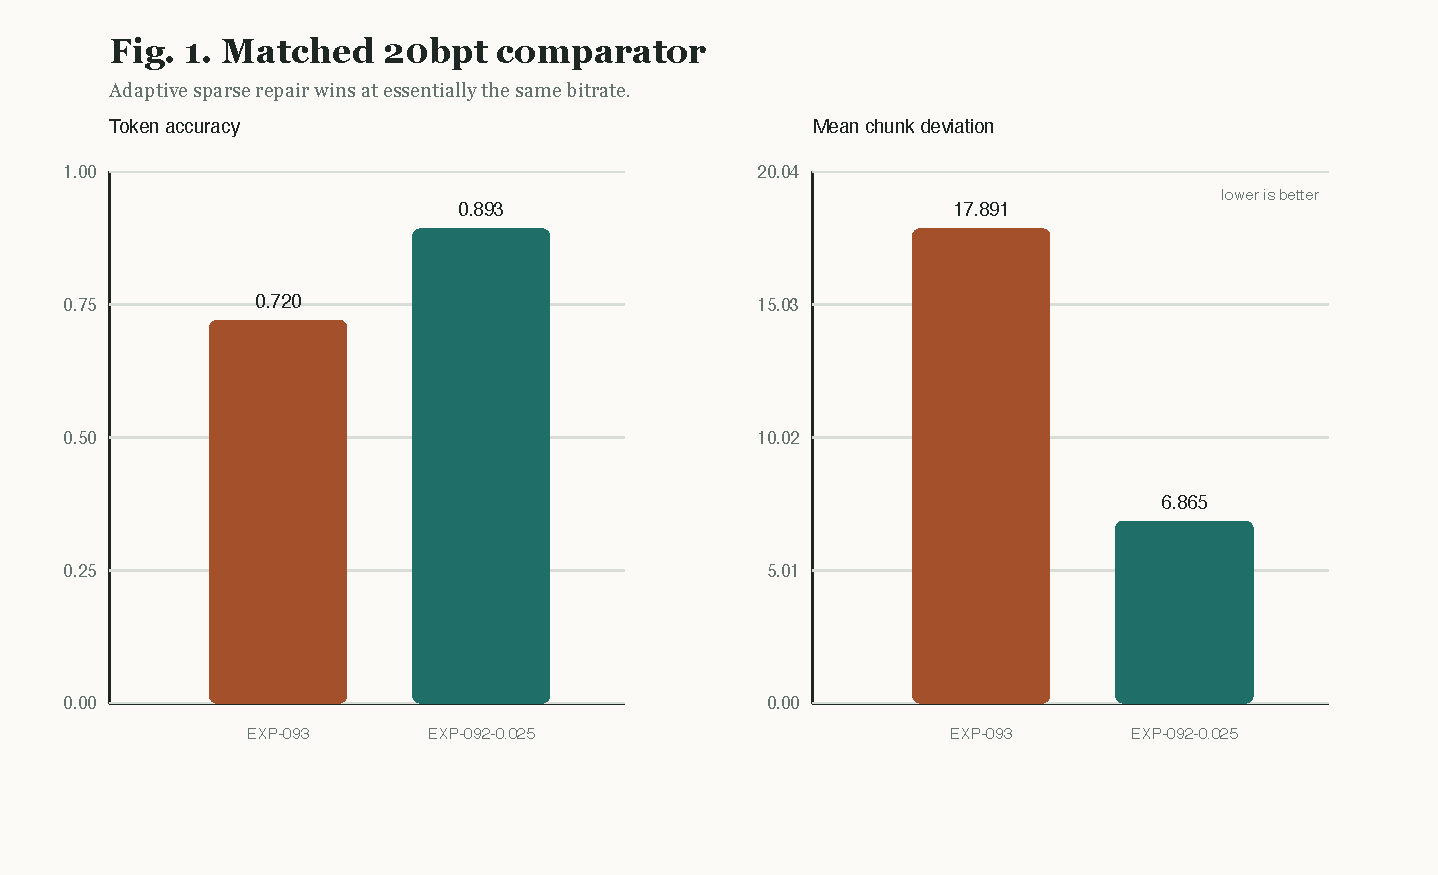
\includegraphics[width=0.95\linewidth]{fig01_matched_20bpt_comparator.pdf}
  \caption{Matched 20 \bitsper\ comparator. Cost-aware sparse repair improves token accuracy and chunk deviation relative to a fixed-rate no-lookup learned compressor at nearly the same bitrate.}
  \label{fig:matched20}
\end{figure}

\begin{table}[t]
\centering
\caption{Matched 20 \bitsper\ result.}
\label{tab:matched20}
\begin{tabular}{lrrrr}
\toprule
Setting & \bitsper & Token acc. & Mean dev. & p90 dev. \\
\midrule
\Exp{093} fixed-rate no lookup & 20.00000 & 0.72045 & 17.89119 & 24.14597 \\
\Exp{092} cost-aware sparse repair & 20.06207 & 0.89274 & 6.86454 & 10.96876 \\
\bottomrule
\end{tabular}
\end{table}

The absolute token-accuracy gain is 0.17229, and mean chunk deviation falls by 11.02665 tokens per 64-token chunk. The fixed-rate baseline is healthy rather than collapsed: its bit density is 0.48766. The gap therefore supports the claim that the gain comes from where lexical precision is spent, not only from how many bits are spent.

\subsection{Rate-Distortion Frontier}
Figure~\ref{fig:frontier} places the main experiments on a shared rate-distortion plot. Lower chunk deviation at comparable \bitsper\ is better.

\begin{figure}[t]
  \centering
  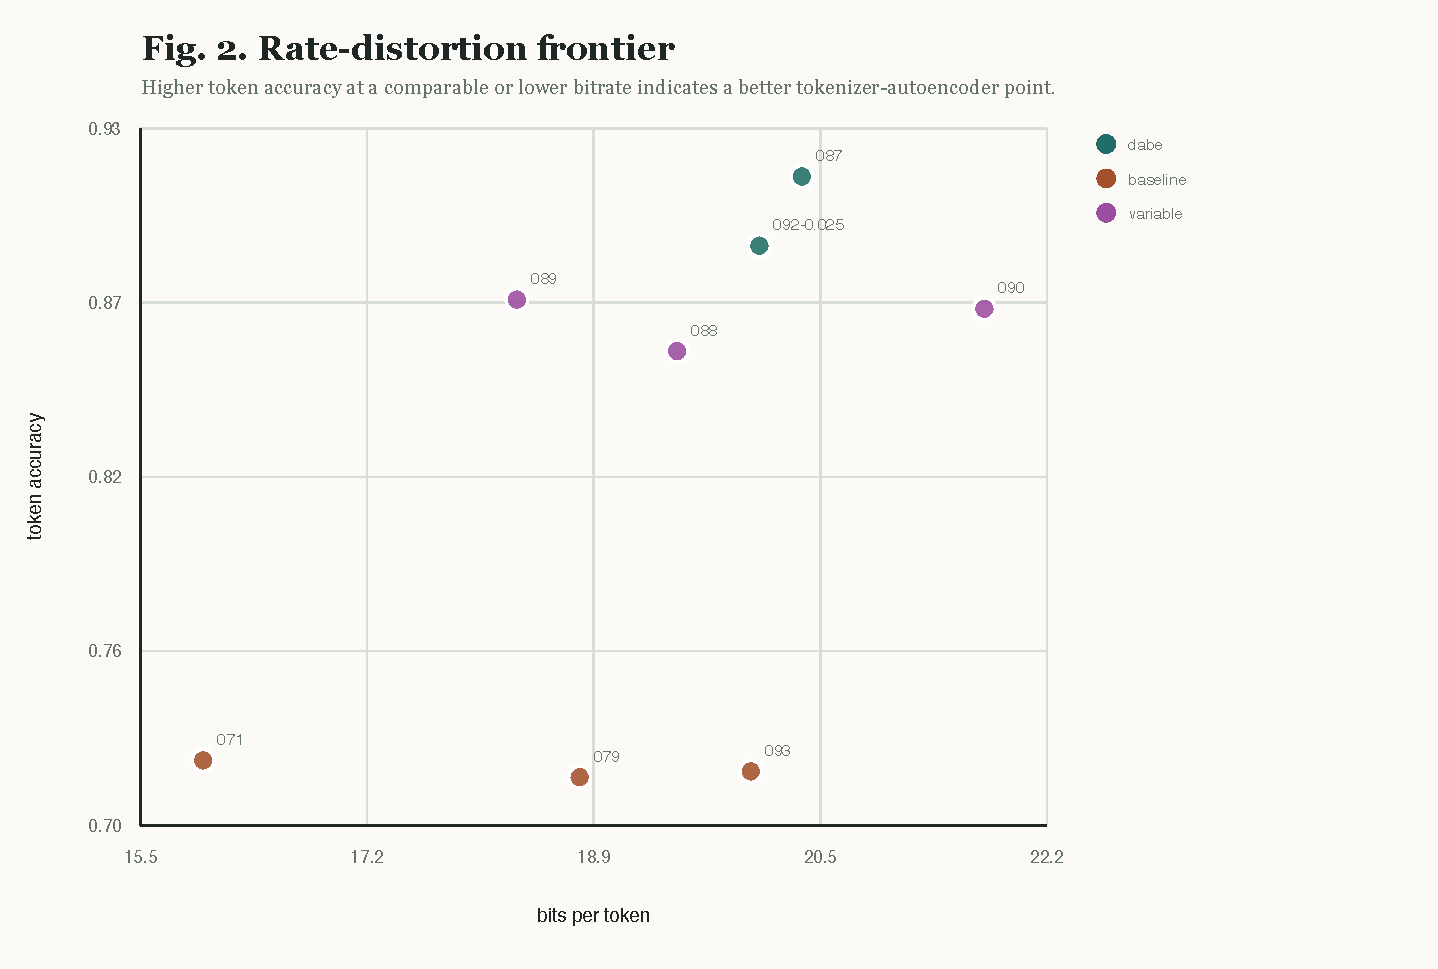
\includegraphics[width=0.95\linewidth]{fig02_rate_distortion_frontier.pdf}
  \caption{Rate-distortion frontier across fixed-rate baselines, sparse lookup models, cost-aware points, and variable-window ablations. Fixed chunks plus sparse repair form the strongest current frontier.}
  \label{fig:frontier}
\end{figure}

The best quality anchor is \Exp{087}, with 0.91547 token accuracy and 5.41007 mean chunk deviation at 20.37236 observed \bitsper. The best lower-cost knee is \Exp{092} with slot cost 0.025, which reaches 0.89274 token accuracy and 6.86454 mean chunk deviation at 20.06207 observed \bitsper.

\subsection{Cost-Knee Replication}
\begin{figure}[t]
  \centering
  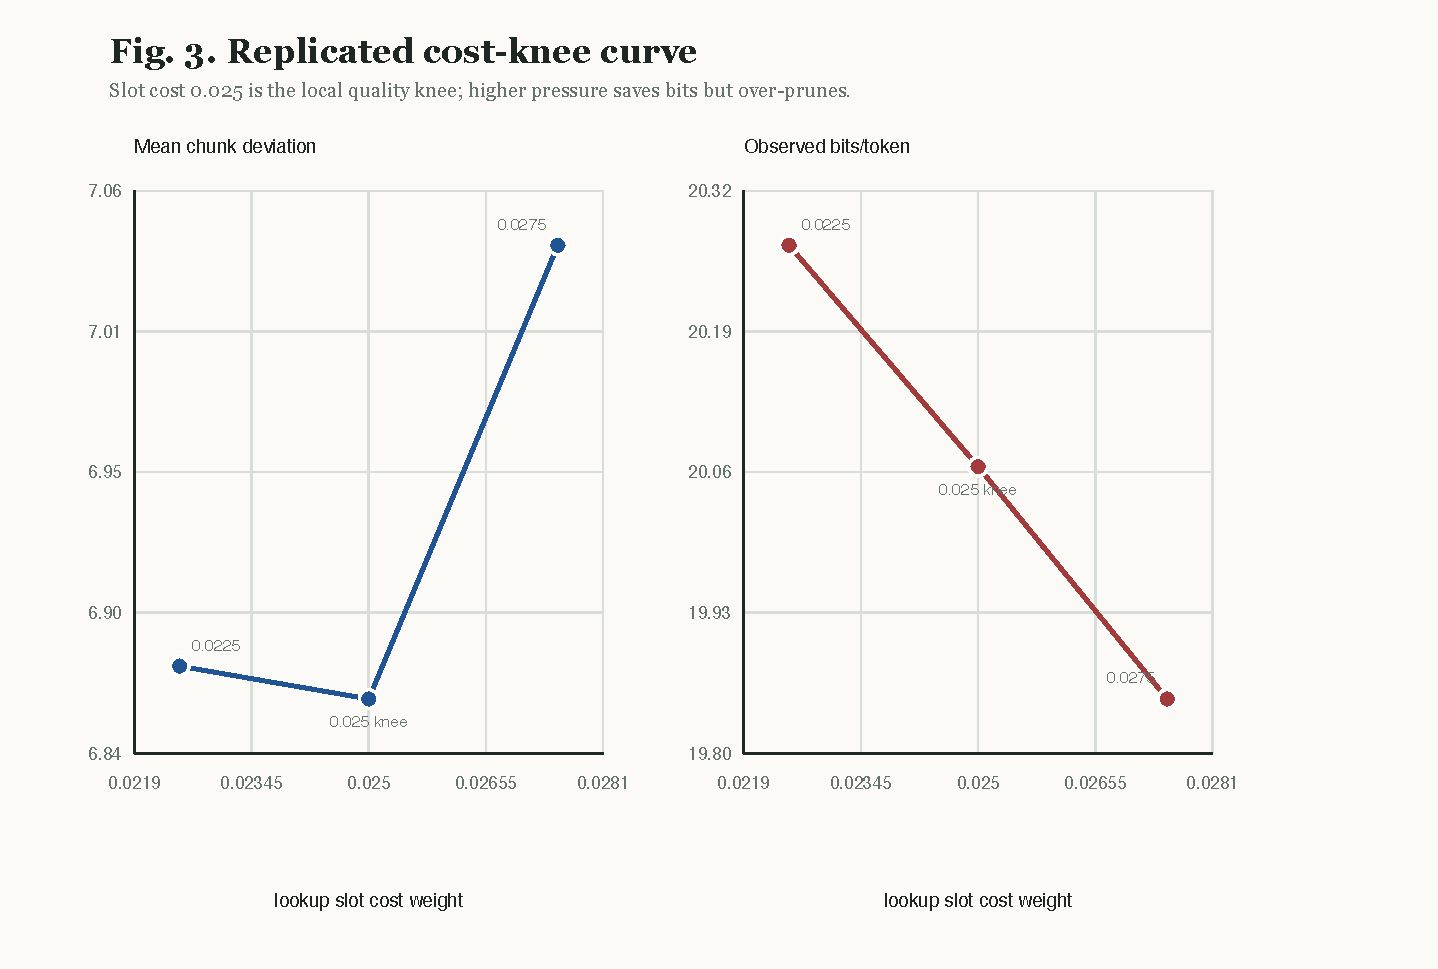
\includegraphics[width=0.95\linewidth]{fig03_cost_knee_curve.pdf}
  \caption{Cost-knee curve for lookup-slot cost. The 0.025 setting is the replicated local knee: lower cost spends more without improving quality, while higher cost over-prunes repair.}
  \label{fig:costknee}
\end{figure}

\begin{table}[t]
\centering
\caption{Lookup-slot cost sweep around the local knee.}
\label{tab:costknee}
\begin{tabular}{rrrrr}
\toprule
Slot cost & \bitsper & Active $K$ & Token acc. & Mean dev. \\
\midrule
0.0225 & 20.26545 & 8.10659 & 0.89255 & 6.87713 \\
0.0250 & 20.06207 & 6.63953 & 0.89274 & 6.86454 \\
0.0275 & 19.84857 & 4.54922 & 0.89002 & 7.03849 \\
\bottomrule
\end{tabular}
\end{table}

The cost term is useful but not sufficient by itself. It controls active slot usage, but the quality anchor remains \Exp{087}. This suggests that future gains should improve the router and lookup content at fixed active $K$, rather than simply increasing cost pressure.

\subsection{Adaptive-Budget Ablation}
\begin{figure}[t]
  \centering
  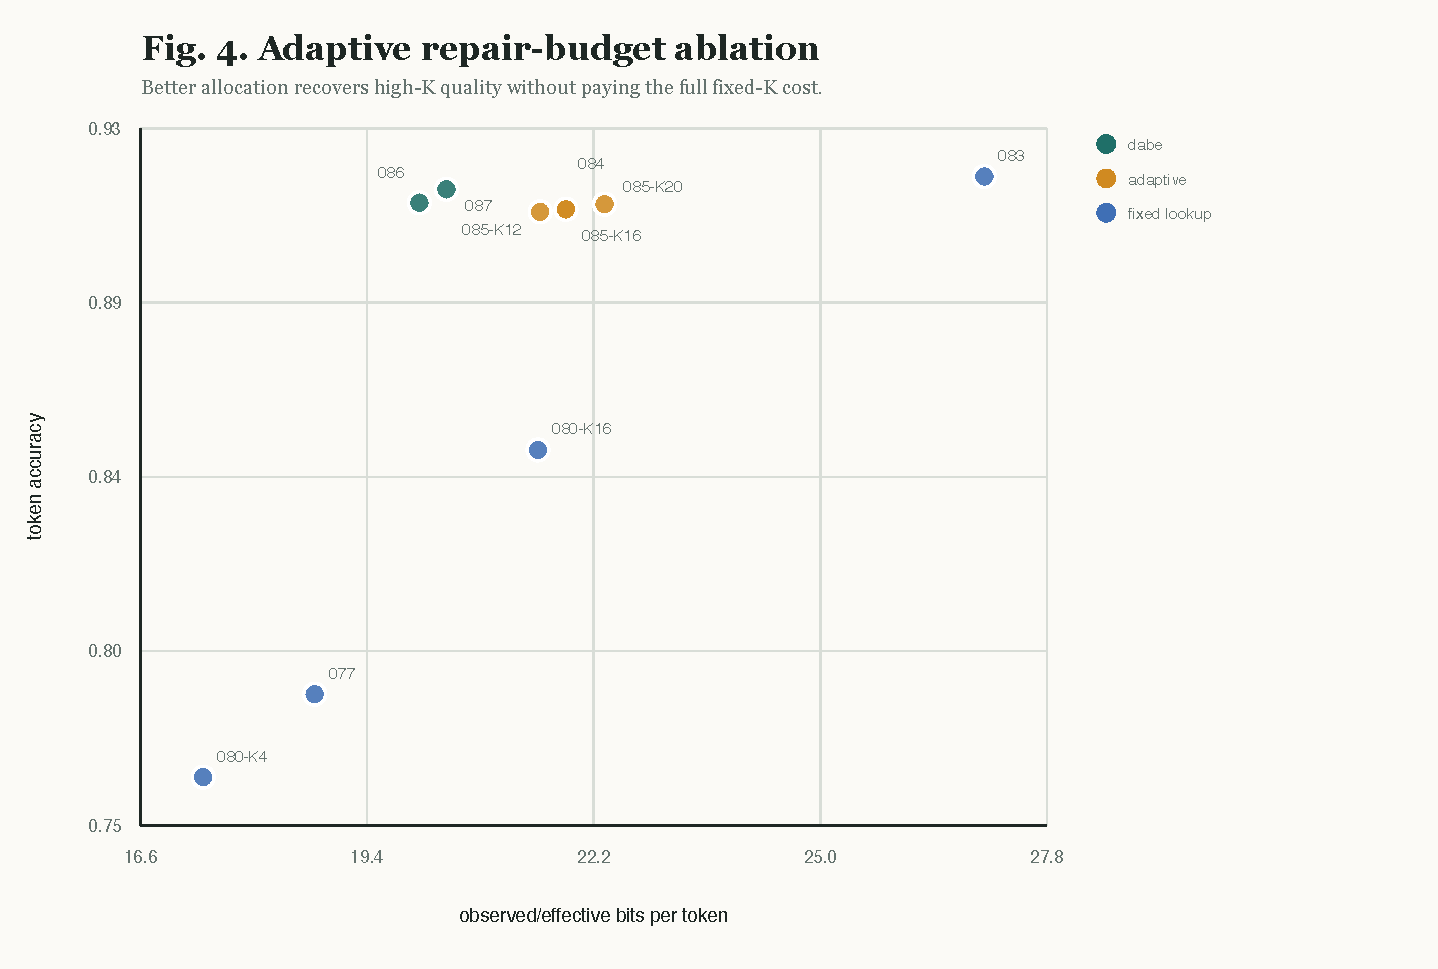
\includegraphics[width=0.95\linewidth]{fig04_adaptive_budget_ablation.pdf}
  \caption{Adaptive-budget ablation. Quality improves as the architecture learns to allocate repair slots more selectively, not merely as raw maximum $K$ increases.}
  \label{fig:budgetablation}
\end{figure}

The ablation path starts with fixed sparse lookup, moves to ranked halting, then adds gist and residual-router supervision. Fixed $K=32$ obtains strong quality at high cost. Ranked halting and gist-residual routing recover much of that quality near the 20--22 \bitsper\ range, motivating the final fixed-chunk plus adaptive sparse repair architecture.

\subsection{Variable-Window Ablation}
\begin{figure}[t]
  \centering
  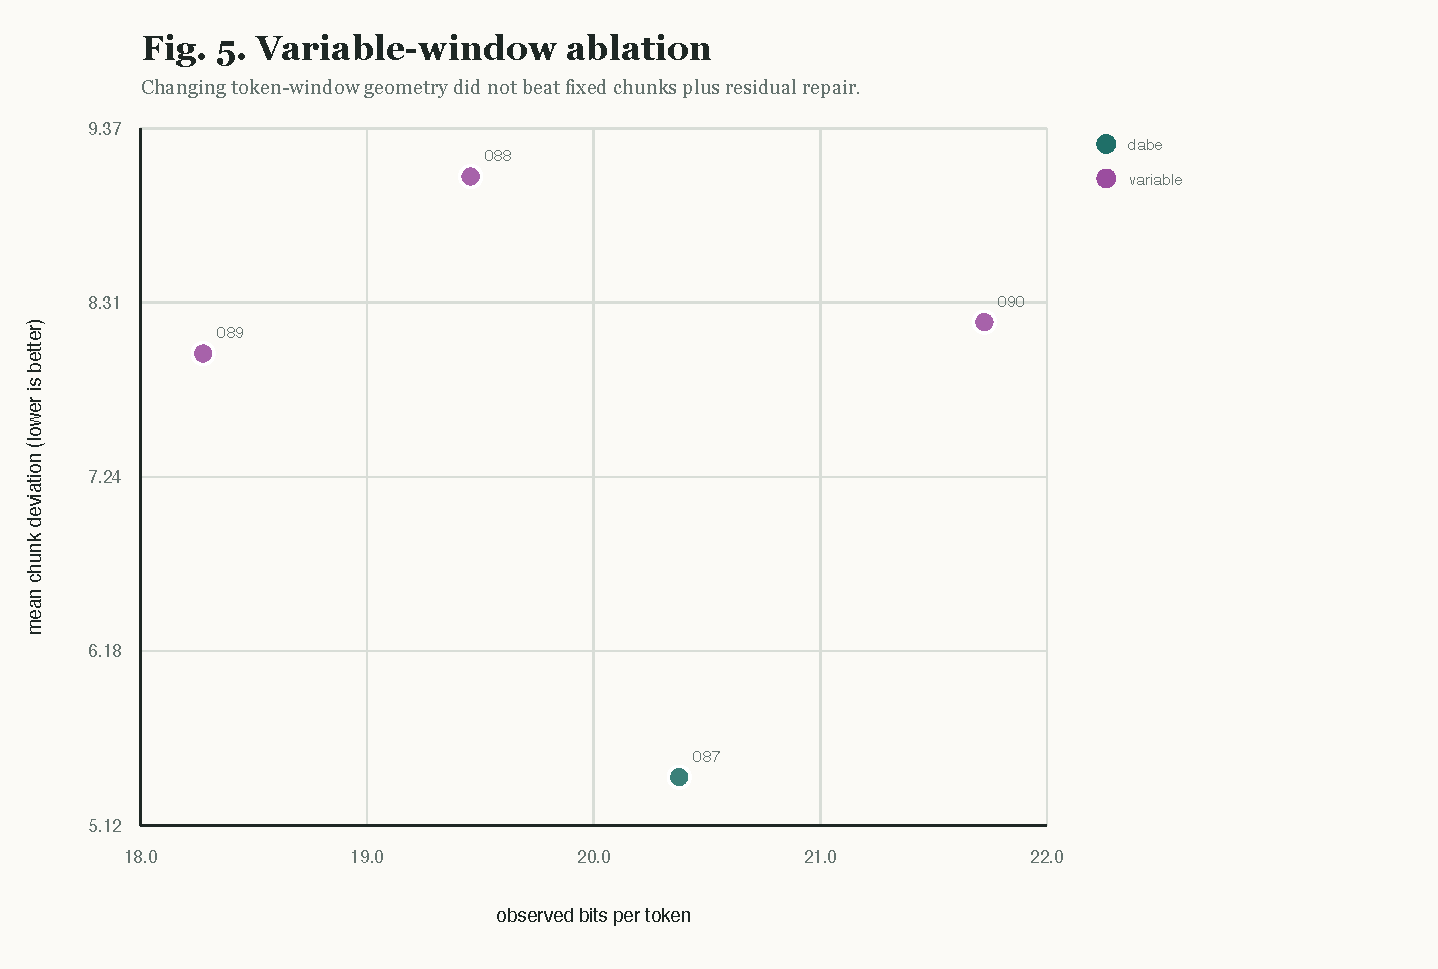
\includegraphics[width=0.95\linewidth]{fig05_variable_window_negative_result.pdf}
  \caption{Variable-window ablation. Sliding token-window geometry underperforms the fixed-chunk sparse-repair anchor.}
  \label{fig:variablewindow}
\end{figure}

\begin{table}[t]
\centering
\caption{Variable-window ablations compared with the fixed-chunk quality anchor.}
\label{tab:variablewindow}
\begin{tabular}{lrrr}
\toprule
Setting & \bitsper & Token acc. & Mean dev. \\
\midrule
\Exp{088} quantile variable windows & 19.46092 & 0.85820 & 9.07550 \\
\Exp{089} action-value variable windows & 18.29175 & 0.87508 & 7.99482 \\
\Exp{090} hard straight-through windows & 21.70567 & 0.87209 & 8.18653 \\
\Exp{087} fixed chunk + residual lookup & 20.37236 & 0.91547 & 5.41007 \\
\bottomrule
\end{tabular}
\end{table}

This ablation narrows the paper's mechanism claim. Adaptive granularity is useful, but in our experiments it belongs in the repair budget rather than in the primary token-window geometry.

\subsection{Active $K$ and Quality}
\begin{figure}[t]
  \centering
  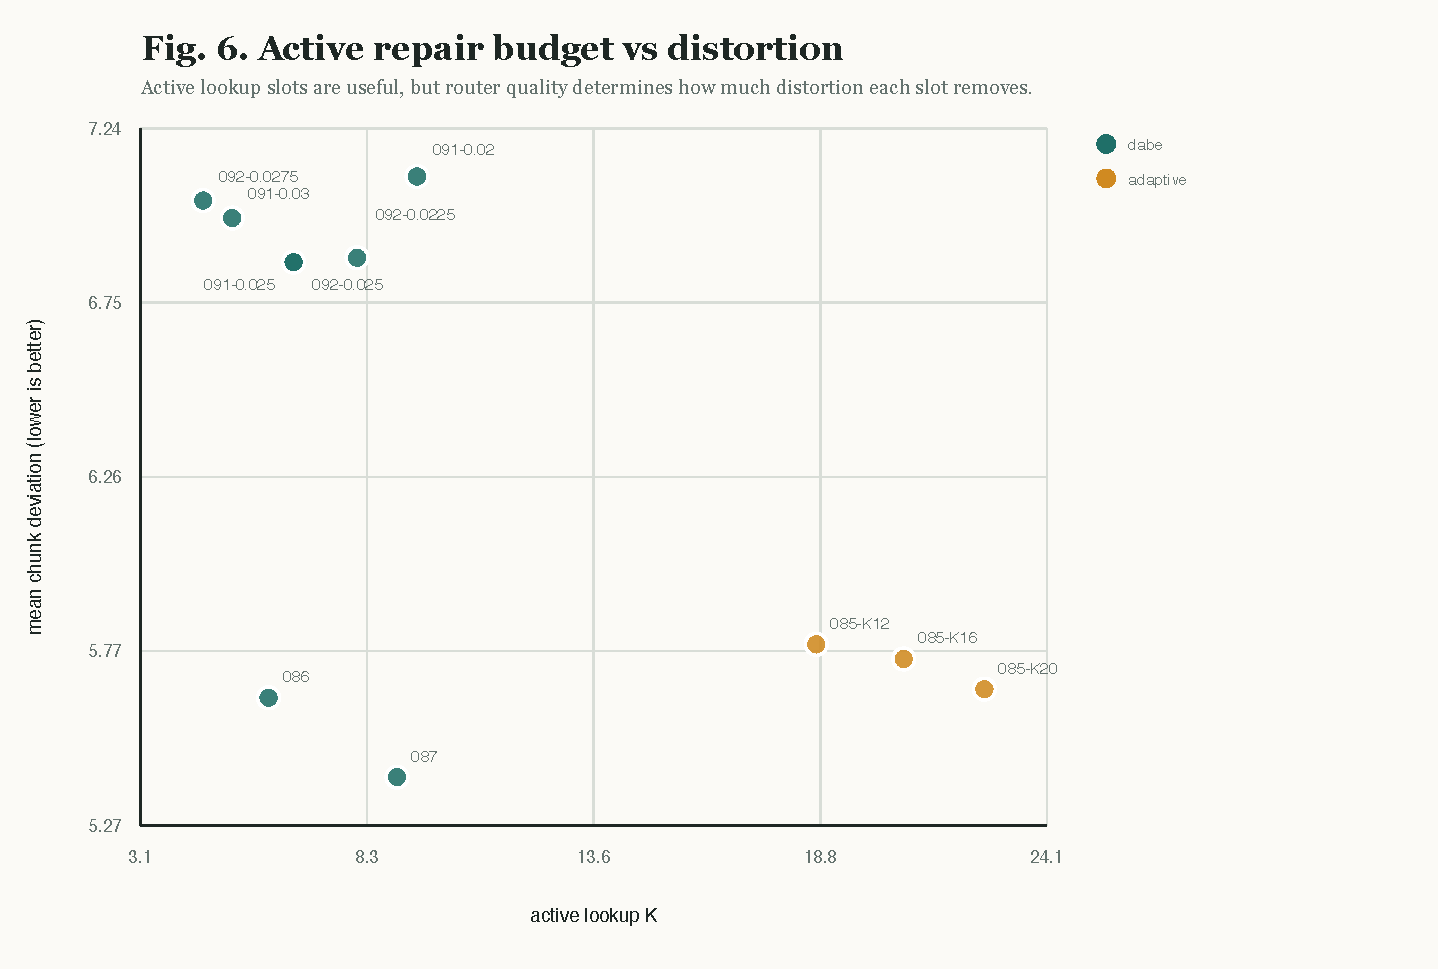
\includegraphics[width=0.95\linewidth]{fig06_active_k_vs_quality.pdf}
  \caption{Active repair budget versus distortion. The best points are not simply the largest active-$K$ points; selective allocation matters.}
  \label{fig:activek}
\end{figure}

Figure~\ref{fig:activek} supports the mechanism interpretation. More active slots often help, but the strongest points are produced by architectures that spend slots selectively. This is the empirical counterpart of Equation~\ref{eq:observed-rate}: the side budget must buy useful lexical repairs rather than simply activate more capacity.

\section{Analysis}
\paragraph{Why sparse repair works.}
The gist path turns the chunk code into a smooth whole-span prior. This is useful for predictable text, but exact token reconstruction is brittle around names, punctuation, dialogue markers, and other locally high-information regions. Sparse repair gives the model an explicit way to allocate lexical precision to these holes. Equation~\ref{eq:chunk-deviation} makes the consequence measurable: the target is not vague semantic similarity, but fewer wrong tokens per chunk.

\paragraph{Why the fixed-rate comparator matters.}
\Exp{093} is the rate-matched comparator that isolates the mechanism. It spends the same budget scale inside a learned chunk autoencoder, but without the sparse lexical repair path. Its much higher chunk deviation shows that uniform capacity is a weak substitute for adaptive repair.

\paragraph{What remains open.}
The cost-aware knee shows a path toward better compression, but it also shows that cost pressure alone diminishes on either side of 0.025. The next architectural question is how to improve lookup correctness and router calibration at a fixed active $K$.

\section{Limitations}
This study is intentionally framed as tokenizer-autoencoder rate-distortion rather than full downstream language-model pretraining. That choice isolates the tokenization mechanism: the experiments measure how chunk codes, sparse repair, and routing policies affect reconstruction before adding the confounds of language-model scale, optimizer schedules, and downstream task selection. The matched 20 \bitsper\ comparison is therefore the central evidence unit for the paper.

The main experiments use TinyStories as a controlled text domain with exact GPT-2-token reconstruction metrics. This setting makes it possible to compare architectural variants under the same token basis, chunk length, training budget, and validation protocol. Domain generalization remains a separate evaluation target; this setting establishes a clean mechanism result that should next be tested on broader corpora, code, multilingual data, and full LM training.

The run plan prioritizes focused, objective comparisons over broad exploratory sweeps. The experiment set includes a matched fixed-rate comparator, a replicated cost-knee neighborhood around \Exp{092}, a quality anchor in \Exp{087}, and direct variable-window ablations. Additional seeds and larger-scale runs would support confidence intervals and scaling laws, but they are not required to interpret the main matched-rate separation.

The current models are rate-distortion tokenizers, not lossless compressors. Exact full-chunk reconstruction remains low, while token accuracy, exact local blocks, and mean chunk deviation improve substantially with sparse repair. This is the correct operating point for the paper's claim: \dabe\ demonstrates that adaptive repair allocation can sharply reduce reconstruction distortion at a matched observed bitrate.

\section{Conclusion}
\dabe\ studies tokenization as a learned rate-distortion problem over fixed text chunks. The strongest result is not obtained by changing token-window geometry, but by keeping a stable 64-token chunk and adapting a sparse lexical repair budget over it.

The matched comparison between \Exp{093} and \Exp{092} is the central result: a healthy fixed-rate no-lookup learned tokenizer at 20.0 \bitsper\ reaches 0.72045 token accuracy and 17.89119 mean chunk deviation, while cost-aware \dabe\ reaches 0.89274 token accuracy and 6.86454 mean chunk deviation at 20.06207 observed \bitsper. This shows that total bit budget alone does not explain the gain.

The broader ablation story is consistent. Fixed sparse lookup improves over no-lookup codes; ranked halting recovers much of fixed $K=32$ quality at lower observed bitrate; the gist-residual architecture improves repair allocation further; and variable token-window geometry fails to beat fixed chunks plus repair. The architectural implication is clear: for learned tokenizers, adapt the repair budget before adapting the token window.

\bibliographystyle{plain}
\bibliography{references}

\end{document}
